\chapter{Background}
\label{cha:background}

In this chapter, we analyze the state of the art of all the relevant fields
involved in this work. Business Process Management, covered in
Section~\ref{sec:background_bpm} is where the main contribution of this work
lies in, since we aim to define a new business process modeling technique.
Natural Language Processing, covered in Section~\ref{sec:background_nlp} is used
extensively in our work in order to automatically extract the relevant
information out of unstructured business process description. Finally,
Section~\ref{sec:background_nlp4bpm} presents \emph{NLP4BPM}, a project
developed in our research group which is very closely related to the work
presented.


%Finally, there are several parallels that can be drawn between ATD, defined in
%this work, and ontologies for the definition of business processes, such as the
%Process Specification Language (PSL). Section~\ref{sec:background_ontologies}
%covers the basic concepts in the field of knowledge representation with
%ontologies.


\section{Business Process Management}
\label{sec:background_bpm}

%\todo{I should explain simulation somewhere in this section.}
%Describe importance and goals of the BPM field.

In large companies and organizations coordination between multiple actors
involved in \textit{business processes} is very important for correct
operations. Business process management is a field of research focused in how to  
\textit{communicate}, \textit{document}, \textit{analyze} and \textit{enhance}
business processes.

Business Process Management approaches processes at three different
levels\cite{mendling2017challenges}:

\begin{description}
  \item[Multi Process Management]{ focuses on the identification of major
      processes of an organization and their priorization. This task
      involves the inspection of the data repositories of a company, such as
      \emph{Data Warehouses}, in order to discover and extract process
      what are the relevant business processes.}
  \item[Process Model Management]{ is concerned with the management of a single
      Business Process Model. This involves \emph{discovering} the process and
      creating a \emph{process model} using some kind of process model notation,
      as well as implementing the necessary \emph{monitoring} tools in order to
      \emph{control} the process.}
  \item[Process Instance Management]{ deals with the actual execution of
      process: \emph{Planning} how the tasks are going to be executed,
      \emph{monitoring} the process during its execution and \emph{adapting} the
      process if problems are detected.}
\end{description}


BPM is a very wide area of research, with several sub-fields focusing on
different aspects of business processes. From very theoretical research based on
Petri net theory\cite{citation needed}, to empirical psychological research
about the \emph{process of process modeling}\cite{citation needed}. The project
described in this Master Thesis is englobed in an emerging
field\cite{vanderaa2018challenges} in BPM, focused in the relation between human
natural language and the formal methods found in other fields of research, such
as \emph{Process Mining}\cite{van2016process}.


%Among all the different sub-fields of BPM, \emph{Process Mining} deserves
%special attention. Process Mining, defined by one of its greatest proponents as
%\emph{Data Science in Action}\cite{van2016process}, is a research area focused on
%developing techniques that allow for extracting business process information
%from event logs. An event logs is sequence of labeled events that is typically
%extracted from the data repositories of an organization (e.g. a \textit{Data
  %Warehouse}). At least, an event should contain a timestamp and some kind of
%description, but more information can be added such as the resources involved,
%the cost for the particular action executed or the actors involved in its
%execution. For instance, in a bank process for evaluating the credit score of a
%client, the event $\langle timestamp, activity, role, actor \rangle = \langle
%1527612256, background\_check, Manager, John \rangle$
%indicates that at some point in time, John (the Manager) ran a background check
%for a client. The following problems are examples of the focus of the research
%in Process Mining:

%\begin{itemize}
%\item Discovering a Business Process Model, given an event log
%\item Generating a simulated event log, given a business process model
%\item Finding an alignments between event logs and business process models, or
  %between themselves
%\item Enhancing or correcting existing process models by analyzing the event logs
%\item Detecting the \emph{conformance} of an event log to a business process model
%\item Analyzing the behavioural (i.e. control flow) patterns in a business
  %process model or an event log
%\end{itemize}


\subsection{Business Process Notations}

%Make a short description of various PM notations, focus on bpm

%Also mention: BPEL, and other BPMN-like old notations and Declarative langauges such as DECLARE or DCR graphs

%Add a note on what is representational bias and how it affects PM notations

This Master Thesis presents an alternative to conventional Business Process
Notations (BPN). In the literature, one can find numerous approaches to BP modelling
techinques. In their survey\cite{10.1007/978-3-540-72035-5_7}, Ruopeng Lu and
Shazia Sadiq, classify Business Process Notations in graph-based and rule-based.

Graph-based BPN represent business processes as a control flow graph. They are
heavily inspired, and usually convertible to Petri Nets\cite{lohmann2009petri},
a formal mathematical model usually employed to describe distributed systems. In
graph-based BPN, the process is described as a sequence of linked nodes,
indicating sequential, alternative or concurrent execution paths. To this day,
the most prominent graph-based business process notation is the Business Process
Model and Notation (BPMN)\cite{chinosi2012bpmn}, with its first version
published in 2011. However, before BPMN's quick rise in popularity, the Business
Process Execution Language (BPEL) had the most widespread usage. Several other
alternatives like YAWL \cite{van2005yawl} have been proposed both from the
academics and the industry. Figure~\ref{fig:bpn_comparison_graph} shows a
comparison between the three aforementioned graph-based business process
notations. Despite their differences, there is a minimum subset of elements that
almost all of them have in common. \textit{(i)} The notion of activity, which is
a task to be executed in the process, usually containing a text label in order
to provide semantics to the process. \textit{(ii)} The \emph{XOR} split, which
branches the execution in two alternative paths, and only one of them may be
executed for any process instance. \textit{(iii)} The \emph{AND} split, which
branches the execution into two concurrent paths, the execution of which can be
interleaved arbitrarily.



\begin{figure}[htb]
  \begin{minipage}{.65\textwidth}
    \centering
    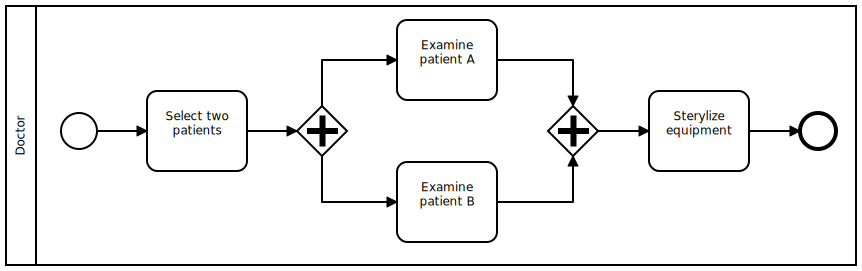
\includegraphics[width=\textwidth]{figures/bpn_comparison/bpmn}
    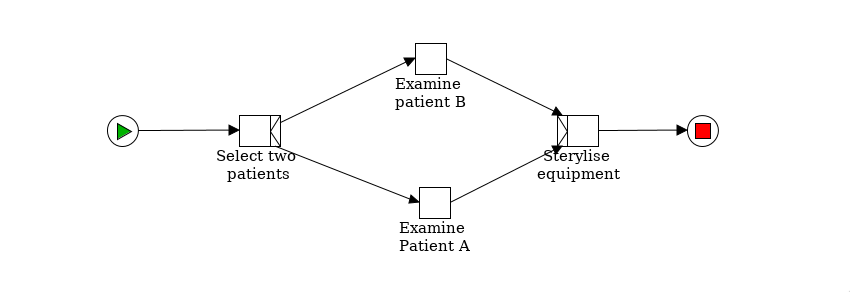
\includegraphics[width=\textwidth]{figures/bpn_comparison/yawl}
  \end{minipage}
  \hfill
  \begin{minipage}{.34\textwidth}
    \centering
    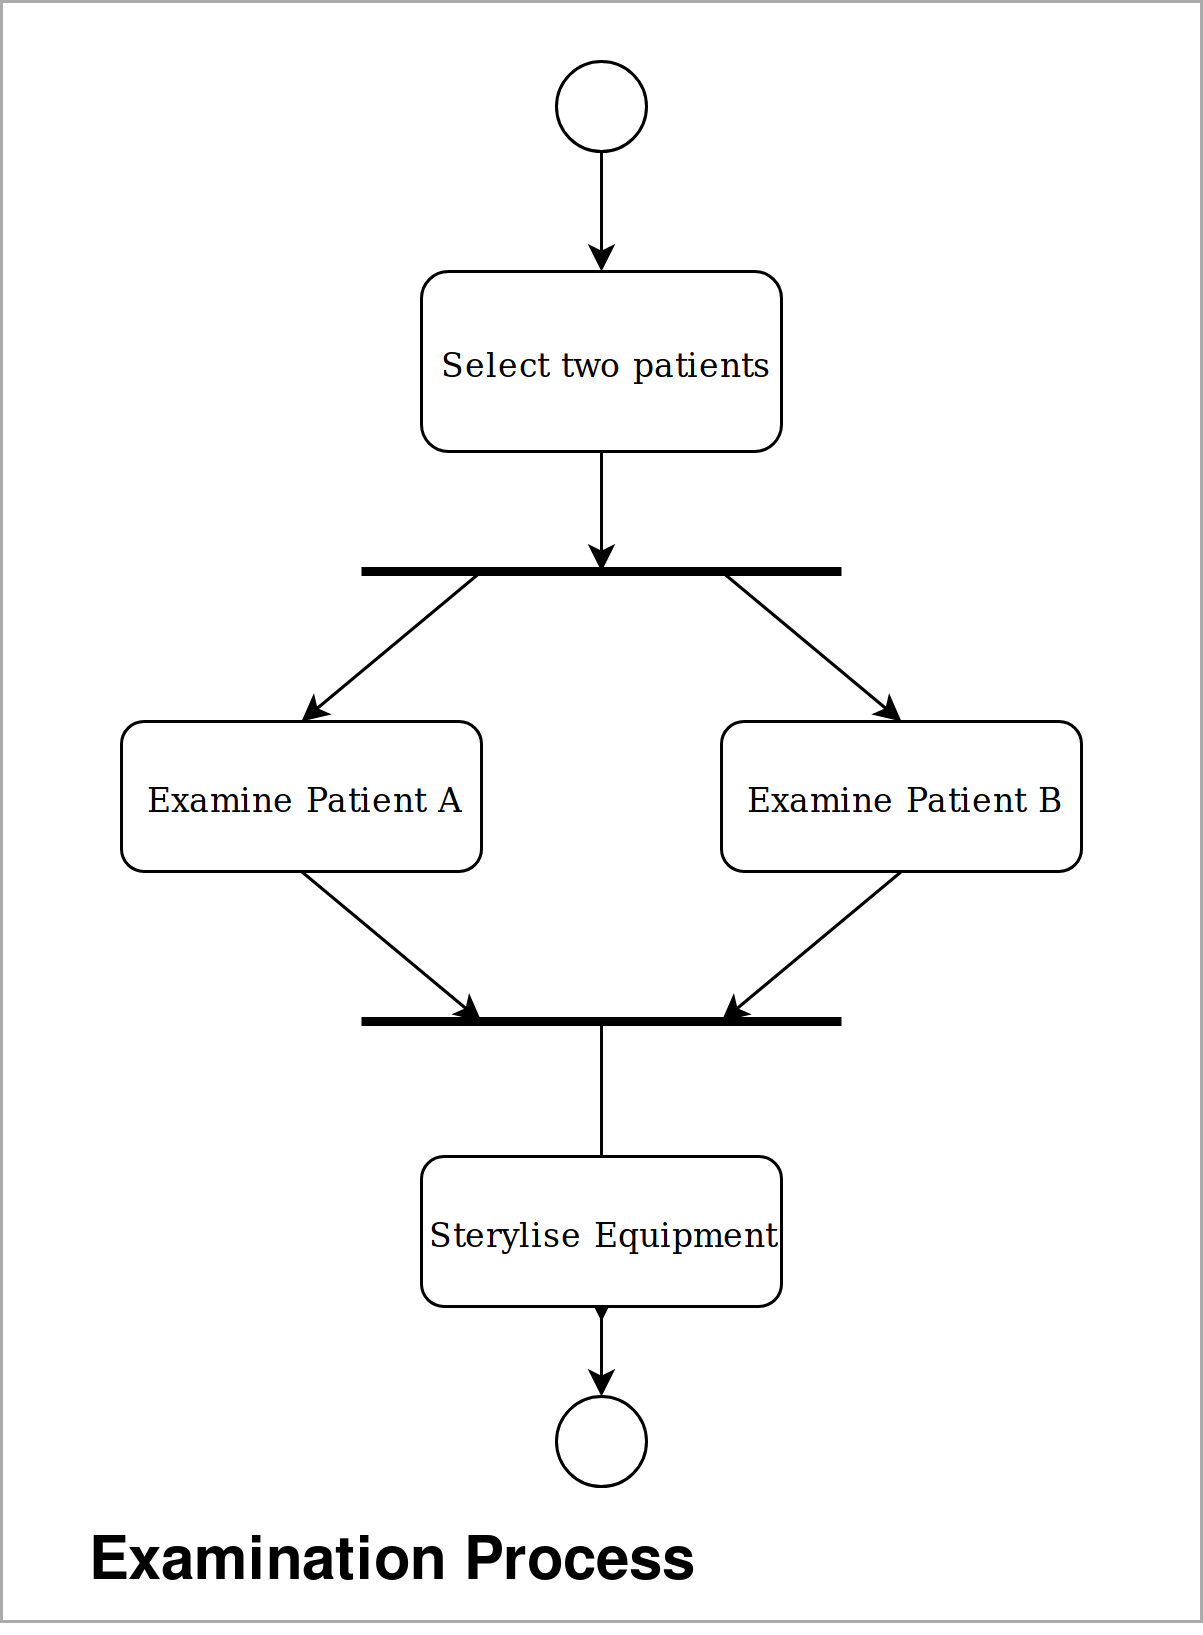
\includegraphics[width=\textwidth]{figures/bpn_comparison/BPEL}
  \end{minipage}
  \caption{Example process in different graph-based execution languages: BPMN (top-left)
     YAWL (bottom-left) BPEL (right).}
  \label{fig:bpn_comparison_graph}
\end{figure}

Rule-based BPN express the process model as a set of rules. In most rule-based
systems, the rules are expressed as restrictions (e.g. ``A request form can only
be sent by a manager''). The main difference of these systems with respect to
Graph-based alternatives is that they allow more flexible behaviour to be
described in a more natural way, at the cost of higher verbosity and being more
error prone. For instance, consider a variation of the process described in
figure \ref{fig:bpn_comparison_graph} where the order of the examinations is
irrelevant, but it is mandatory for the doctor to sterylise the medical
equipment between the two. In graph-based systems, duplication of activities
cannot be avoided to express the semantics of this rule. On the other hand, most
rule-based systems can introduce the rule that task $sterylize$ must always
happen between two examinations.

\section{Natural Language Processing}
\label{sec:background_nlp}

\emph{Natural Language Processing} is a field of artificial intelligence which
addresses the interactions between computers and human languages. NLP focuses on
many problems at different levels of abstraction, from the purely linguistic
ones like morphosyntactic analysis or determining the part-of-speech of words
to very challenging tasks such as the automatic summarization of news articles.

Those tasks that go beyond parsing at a syntactic level and focus on the
\emph{semantics} of written text are usually classified under the field of
\emph{Natural Language Understanding} (NLU). The focus in NLU is to build
complete semantic representations of texts in a machine-friendly format. It is
thus an AI-complete\cite[Section 1]{ai_completeness} problem, since text are
addressed to human readers under the assumption of common sense and world
knowledge: Things very difficult to encode in a computer program. 

NLP techniques are applied to address a variety of use cases in the context of
Business Process Management. Several of these focus on the text contained in
process models themselves. This includes a variety of works that focus on the
quality of process model labels, for example by detecting violations of labeling
conventions~\cite{becker2009,leopold2013detection,vandervos1997verification},
inconsistent use of terminology~\cite{koschmider2007}, or common modeling
errors~\cite{gruhn2011detecting}. Other approaches use NLP to augment process
models with semantic or ontological
information~\cite{leopold2015towards,francescomarino2009supporting,born2007userfriendly}.

Other use cases involve texts that exist outside of process models. Several
approaches extract process models from different kinds of text, such as from use
cases~\cite{sinha2010use}, group stories~\cite{gonccalves2009business}, or
methodological descriptions~\cite{epure2015automatic},  while others take
general textual process descriptions as
input~\cite{ghose2007process,friedrich2011process}. However,  these approaches
have been found to produce inaccurate models, which require extensive manual
revision~\cite{selway2015formalising}. Other use cases involving texts include a
technique that considers \textit{work instructions} when querying process
repositories~\cite{leopold2017searching} for conformance checking against
textual process descriptions~\cite{vanderaa2018checking}.


\subsection{Steps of Language Analysis}

 The NLP processing software used in this work is
 FreeLing\footnote{\url{http://nlp.cs.upc.edu/freeling}}~\cite{PadroS12}, an
 open--source library of language analyzers providing a variety of analysis
 modules for a wide range of languages. More specifically, the natural language
 processing layers used in this work are:
 
\begin{description}
\item[Tokenization \& sentence splitting:] Given a text, split the basic lexical
  terms (word, punctuation signs, numbers, ZIP codes, URLs, e-mail, etc.), and
  group these tokens into sentences.
\item[Morphological analysis:] For each word in the text, find out its possible
  parts-of-speech (PoS).
\item[PoS-Tagging:] Determine which is the right PoS for each word in a
  sentence. (e.g. the word \textit{dance} is a verb in \textit{I dance all
    Saturdays} but it is a noun in \textit{I enjoyed our dance together}.)
\item[Named Entity Recognition:] Detect named entities in the text, which may be
  formed by one or more tokens, and classify them as \textit{person},
  \textit{location}, \textit{organization}, \textit{time-expression},
  \textit{numeric-expression}, \textit{currency-expression}, etc.
\item[Word sense disambiguation:] Determine the sense of each word in a text
  (e.g. the word \textit{crane} may refer to an animal or to a weight-lifting
  machine). We use WordNet \cite{fellbaum98} as the sense catalogue and synset
  codes as concept identifiers.
\item[Constituency/dependency parsing:] Given a sentence, get its syntatic
  structure as a constituency/dependency parse tree.
\item[Semantic role labeling (SRL):] Given a sentence identify its predicates and the
  main actors in each of them, regardless of the surface structure of the
  sentence (active/passive, main/subordinate, etc. For example, in the sentence
  \textit{John does not want to go}, a SRL would detect two predicates
  (\textit{want} and \textit{go}), and mark that \textit{John} is \texttt{Agent}
  of both. Note that a parser could detect that \textit{John} is the
  \texttt{subject} of \textit{want} but it would not detect that he is also the
  one supposed to \textit{go}.  SRL provides a higher level of abstraction than
  a parser, providing slightly deeper semantic knowledge. E.g. in a passive
  sentence such as \textit{the fish was eaten by the cat}, a SRL system would
  detect an event \textit{eat} with \textit{cat} as \texttt{Agent} and
  \textit{fish} as \texttt{Patient}, i.e. exactly the same that it would extract
  from the equivalent active sentence \textit{the cat eats fish}.
\item[Coreference resolution:] Given a document, group mentions referring to the same entity (e.g. a person can be mentioned in the text as \textit{Mr. Peterson}, \textit{the director}, or \textit{he}.) 
\item[Semantic graph generation:] All the information extracted by the previous
  analyzers can be organized in a graph depicting events (mainly coming from
  predicates in the text), entities (coming from detected coreference groups),
  and relations between them (i.e. which entities participate in which events
  and with which role). This graph can be converted to triples and stored in an
  RDF database if needed.
\end{description}

\subsection{Text Annotations}
\label{sec:background_anns}

Creating annotated versions of texts is usual in NLP field, where many
approaches are based on machine learning. Thus, to train a PoS-tagger, text
where each word has been annotated with its part-of-speech, is required.
Similarly, parsers, semantic role labellers, or coreference resolution systems,
need example texts where this linguistic levels have been annotated by humans.
These annotated corpora are then used to train the NLP analyzers and to
evaluate their performance.

Thanks to this need for annotated data in NLP, convenient tools have been
developed to ease the annotation task. One of them is
\emph{Brat}\cite{stenetorp2012brat}\footnote{\url{http://brat.nlplab.org}}, a
configurable environment that allows the annotation of texts with labelled
spans, and relations. Figure~\ref{fig:brat} shows Brat being used to annotate a
scientific text with very specific concepts from the field of biology.


\begin{figure}[htb]
  \centering
  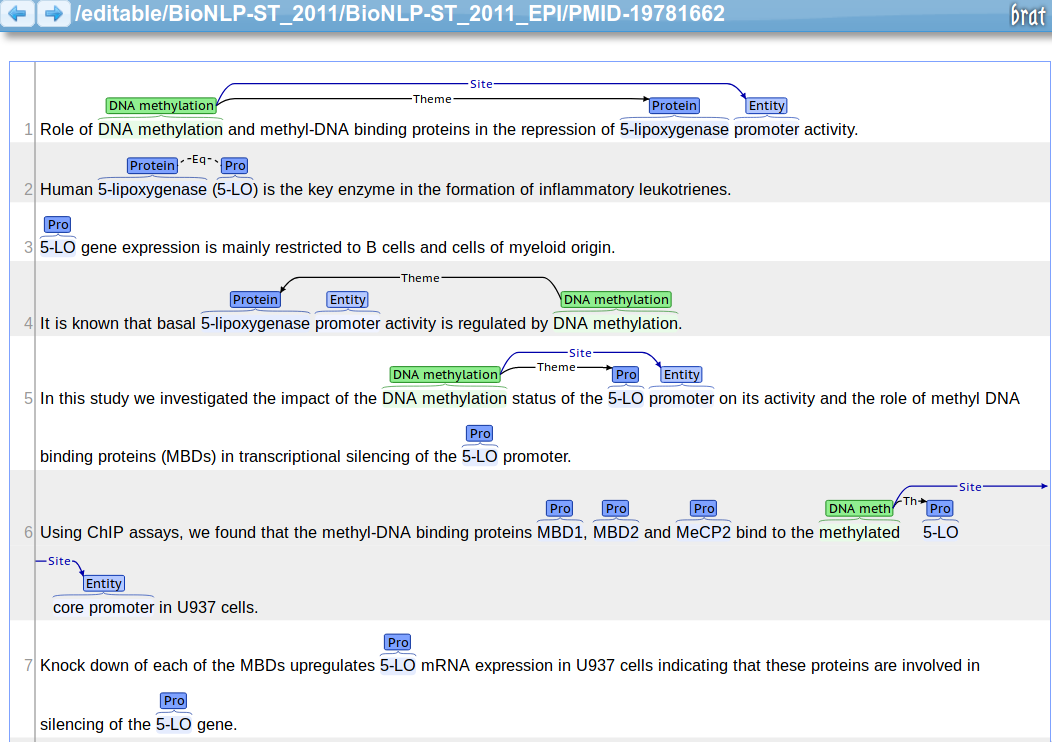
\includegraphics[width=0.8\textwidth]{figures/brat}
  \caption{One of the example annotations provided with the Brat
    annotation tool.}
  \label{fig:brat}
\end{figure}

A more recent alternativ for text annotation are Text Annotation Graphs (TAG)
\cite{DBLP:journals/corr/abs-1711-00529}. TAG is a web-based software which
conceptually improves upon Brat two ways: \textit{(i)} It provides the
functionality of representing complex relationships between text elements,
allowing the definition of relationships between relationships themselves
(semantic hypergraphs). \textit{(ii)} The visualization tool offers a more
ergonomic and flexible representation of the annotated texts, allowing the
repositioning of words, or filtering the view to only show a subset of the
annotated information. Figure~\ref{fig:tag} shows
a text annotated using TAG.


\begin{figure}[htb]
  \centering
  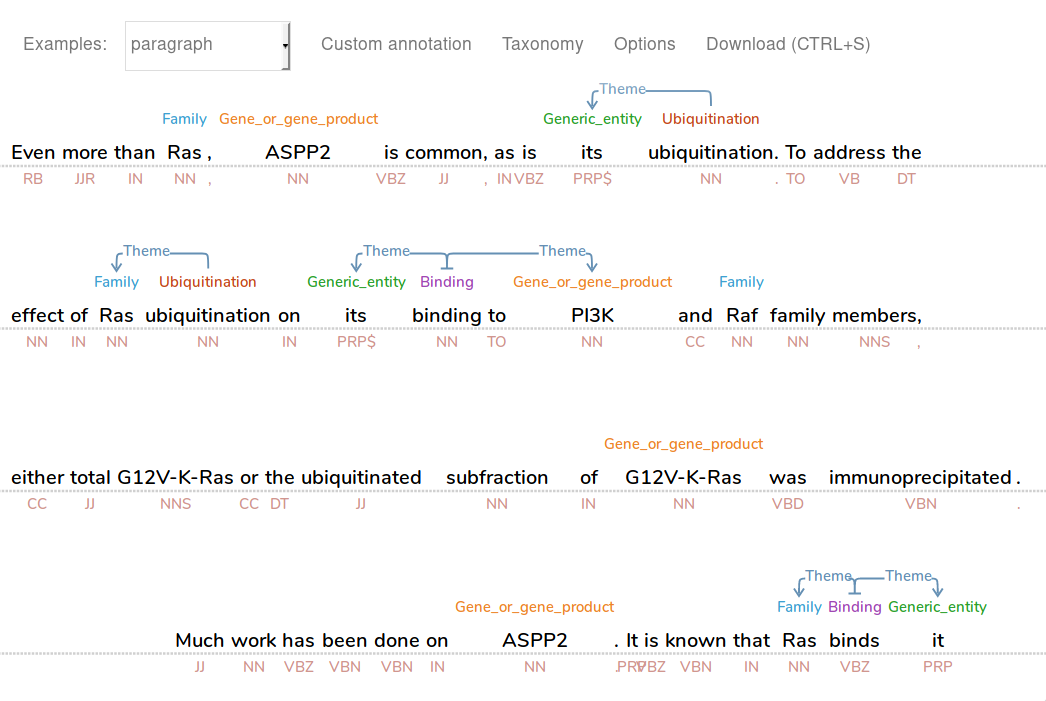
\includegraphics[width=0.8\textwidth]{figures/tag}
  \caption{One of the example annotations provided with the TAG
    annotation tool.}
  \label{fig:tag}
\end{figure}

In this work, we present Annotated Textual Descriptions as a business process
modeling language. ATD are based on text annotations, but its main purpose
differs from the typical use cases of annotations. Ideally, ATD would be
automatically performed by an NLP tool, instead of being used as training data.
However, given the limitations of the current NLP state-of-the-art, we will
resort to a certain amount of human annotation to improve the quality of our
semantic representation. This is discussed in further detail in Chapter~\ref{cha:atd}.

\section{The \emph{NLP4BPM} Project}
\label{sec:background_nlp4bpm}

When multiple business process representations are used inside an organization,
it becomes very important to ensure availability and consistency of the existing
documentation. The \emph{Natural Language Tools for Business Process Management}
(\emph{NLP4BPM}) project, developed by our group in the Polythecnic University
of Catalonia, aims to solve several related problems in this doman.

In \emph{NLP4BPM}, several different approaches are taken in order to aid
organizations in managing multiple representations of processes:

\begin{description}
\item[\emph{Text2BPMN}]{Converting a natural langauge textual description into a
  BPMN business process model.}  
\item[\emph{BPMN2Text}]{Converting a BPMN business process model into a
    human-readable textual description.}  
\item[\emph{BPMNvsText}]{Computing an \emph{alignment} between a model and a
    textual description in order to compare them. An alignment is a mapping
    between tasks in the model and sentences in the text. The implementation
    follows the technique presented in \cite{10.1007/978-3-319-59536-8_26}.}  
\item[\emph{BPMNvsBPMN}]{Computes an alignment between two different BPMN
    models. Here the alignment is between the set of tasks of the two process
    models. The techniques implemented in this module are based on Relaxation
    Labeling algorithms}  
\item[\emph{BPMN2ChatBot}]{Converts a BPMN diagram into an interactive chat bot
    that guides a user throughout the process execution.}
\end{description}

The different techniques are developed as independent modules and unified under
the same graphical interface, which is presented in a user-friendly manner. The
tool is available online at \url{http://nlp4bpm.cs.upc.edu/}.
Figure~\ref{fig:nlp4bpm_example} shows a screenshot of the web user interface.

\begin{figure}[htb]
  \centering
  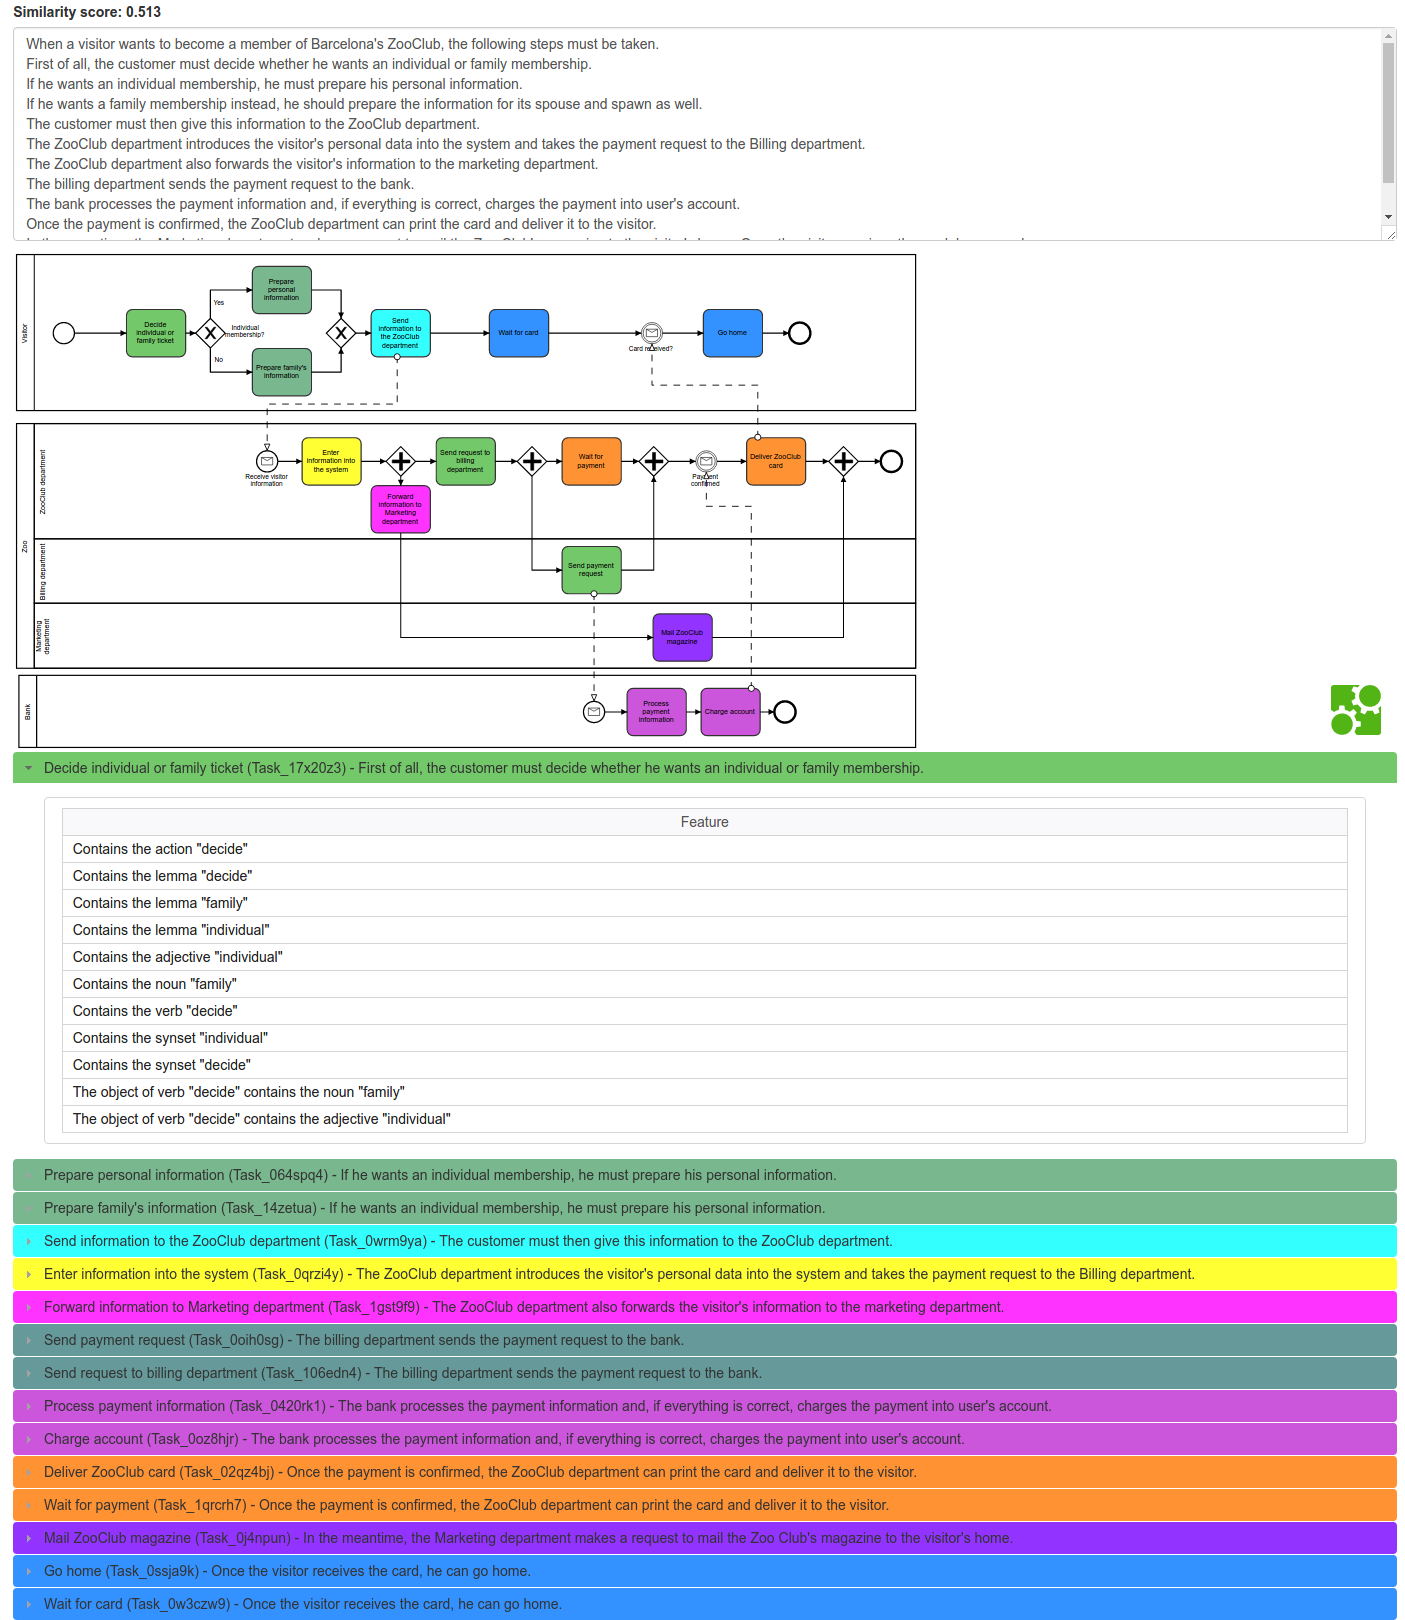
\includegraphics[width=0.8\textwidth]{figures/nlp4bpm}
  \caption{Example execution of the BPMNvsText module at the NLP4BPM web
    interface.}
  \label{fig:nlp4bpm_example}
\end{figure}

One of the common elements in the \emph{NLP4BPM} project is the use of
\emph{FreeLing}, and particularly of \emph{FreeLing}'s \emph{semantic graphs} in
order to extract semantic information from both texts and BPMN labels. A
semantic graph is an abstract representation of a document where entities (e.g.
people, objects) are represented as nodes, and joined by relations, such as the
\emph{temporal adjunct}, which joins an action with the words that describes the
particular time during which it is performed, or the \emph{manner adjunct},
which indicates the way in which the action is performed instead.

One of the goals of this Master's thesis is to link Annotated Textual
Descriptions, the main contribution presented in this work, with FreeLing
semantic graphs. This will allow using ATD in order to improve the robustness of
the algorithms presented above without having to modify them.
Chapter~\ref{cha:atdlib} describes in more detail how this is achieved.

%\section{Ontologies}
%\label{sec:background_ontologies}
